\documentclass[11pt,a4paper]{article}

\usepackage[utf8]{inputenc}
\usepackage[german]{babel}
\usepackage[T1]{fontenc}
\usepackage{helvet}
\renewcommand{\familydefault}{\sfdefault}
\usepackage[left=2cm,right=2cm,top=2cm,bottom=2cm]{geometry}
\usepackage{csquotes}
\MakeOuterQuote{"}
\usepackage{graphicx}
\graphicspath{ {./src/} }

\renewcommand{\refname}{Referenzen}
\renewcommand{\figurename}{Abbildung}
\renewcommand{\tablename}{Tabelle}

\title{Medical Assistent}
\author{Adrian Locher, Jason Benz}
\date{\today}


\begin{document}
\pagenumbering{gobble}
\maketitle
\tableofcontents
\newpage

\pagenumbering{arabic}

\section{Einleitung}
    \subsection{Motivation}
        \paragraph{}
            Die Frage, ob ein Arzt besucht werden soll, ist häufig ein Dilemma.
            Einerseits will man nicht diejenige Person sein, welche bei unbedenklichen Symptomen
            überreagiert, andererseits könnten sich die Symptome verschlimmern und vielleicht
            hätte der Arztbesuch das Problem frühzeitig beheben können. Dazu kommt die
            Krankenversicherung, welche einen Teil der anfallenden Kosten übernimmt und eher ein Argument
            für einen Arztbesuch ist. Aber aus Sicht der Krankenkasse verursacht jede überflüssige
            Konsultation des Arztes unnötige Kosten für die Allgemeinheit.
            
        \paragraph{}
            Eine ganz andere Bedeutung hat dieses Dilemma ausserdem seit dem Anfang
            der Covid-19 Situation. Ärzte und anderes Gesundheitspersonal, gelten als besonders
            stark ausgelastet. Auf der Kehrseite hingegen, sollte man bei Covid-19-artigen Symptomen
            auch nicht zögern und sich testen lassen. Welche Symptome nun genau als "Covid-Symptome"
            gelten und welche nicht, ist teilweise sehr unübersichtlich, was die Lage auch nicht
            einfacher werden lässt.

        \paragraph{}
            Das primäre Ziel unseres Projekts ist eine Lösung zu entwickeln, mit der unnötige Arztbesuche
            generell, aber besonders in Situationen wie den aktuellen, vermieden werden können.
            Es ist nicht beabsichtig die allgemeine Zahl der Arztbesuche zu verringern, sondern in
            Grenzfällen bei der Entscheidung zu helfen.
        
        \paragraph{}
            Um dabei auch wirklich das Gesundheitspersonal maximal zu entlasten, besteht unser
            Lösungsansatz nicht aus einer Hotline oder ähnlichem. Ziel ist es ein AI gestützes System zu
            entwickeln, welches ganz ohne menschliche Interaktion auskommt. Mithilfe von
            Googles Dialogflow Plattform, sowie einem interaktiven Java Client, wurde ein Chatbot
            realisiert, der diese Kommunikation übernimmt.


\newpage


\section{Backend}
    \subsection{Übersicht}
        \paragraph{}
        In Abbildung \ref{fig:backEndFlowChart} ist der logische Ablauf, des Dialogflows zu sehen, welcher das
        Backend unseres Chatbots bildet.
        \begin{figure}[h!]
            \begin{center}
                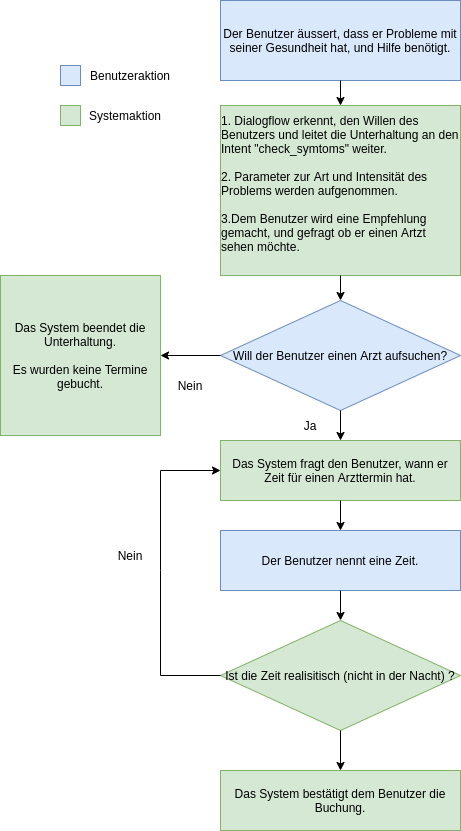
\includegraphics[width=0.65\linewidth]{backendOverview.png}
                \caption{Backend Übersicht-Flowchart}
                \label{fig:backEndFlowChart}
            \end{center}
        \end{figure}


	\newpage


    \subsection{Intents}
        \paragraph{}
            Das Backend ist in vier Intents strukturiert:
            \begin{figure}[h!]
                \begin{center}
                    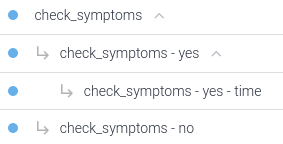
\includegraphics[width=0.4\linewidth]{intents.png}
                    \caption{Dialogflow Intent-Liste}
                    \label{fig:intentslist}
                \end{center}
            \end{figure}

    \subsection{Aufnahme von Symptomen}
        \paragraph{}
            Im ersten Intent des Dialogs \emph{"check\_symtpoms"} wird eine Liste mit Symptomen, sowie ein Schmerzniveau 
            und die Zeitdauer seit dem ersten Erscheinen der Symptome aufgenommen.

        \paragraph{}
            Folgende Trainingssätze wurden für das Auslösen des Intents definiert:
            \begin{itemize}
                \item i have \emph{pain} since \emph{yesterday}
                \item i have \emph{pain}
                \item i need help
                \item should i go to the doctor?
                \item Can you tell me if i should seee a doctor?
                \item Am I sick?
                \item I feel Sick
                \item feel \emph{unwell}
            \end{itemize}
            Die hier \emph{kursiv} geschrieben Wörter werden auf die entsprechenden Parameter gematched.

        \subsubsection{Parameter Entities}
            Um die Symptom-Parameter aufzuzeichnen wurden folgende Parameter und Entities definiert:
            \begin{table}[!h]
                \begin{center}
                    \begin{tabular}{l|l}
                        \textbf{Parameter} & \textbf{Entity}\\
                        \hline
                        SymType & symptom\_type\\
                        SymIntensity & symtom\_intensity\\
                        SymDuration & System.Date
                    \end{tabular}
                    \caption{Paramter und Entities}
                    \label{tab:tabelleParamsUndEntities}
                \end{center}
            \end{table}


			\newpage
            
            
            \paragraph{}
                \textbf{symtom\_type} hat einen Wertebereich von: pain, unwell, sick, fever, cough, loss of taste, 
                chestpain, tiredness und shortness of breath mit jeweils drei bis vier Synonymen.
            
            \paragraph{}
                \textbf{symtom\_intensity} hat einen Wertebereich von 1 bis 5. Diese können jeweils in Worten 
                (\emph{z. B. "One", "Eins" usw.}) oder als Zahl (\emph{z. B. 1}) angegeben werden.
            
            \paragraph{}
                \textbf{System.Date} ist ein vorgefertigtes Entity mit einem Wertebereich, welcher beliebige Kalenderdaten
                enthalten kann.
                
    \subsection{Auswertung der Symptome}
        \paragraph{}
            In einem zweiten Schritt geht es nun um die Auswertung der Angaben, damit dem Patienten Tipps zum weiterem Verhalten
            gegeben werden können. Die Auswertung findet am Ende des Intents statt, indem ein Webhook aufgerufen wird.
            Hier ist als Antwort auf dem entsprechenden Intent \emph{"check\_symptoms"} eine Funktion \emph{"checkSymptoms"}
            (siehe: Abbildung \ref{fig:checksymptomsfunction}) registriert.
	        \begin{figure}[h!]
    	        \begin{center}
        	        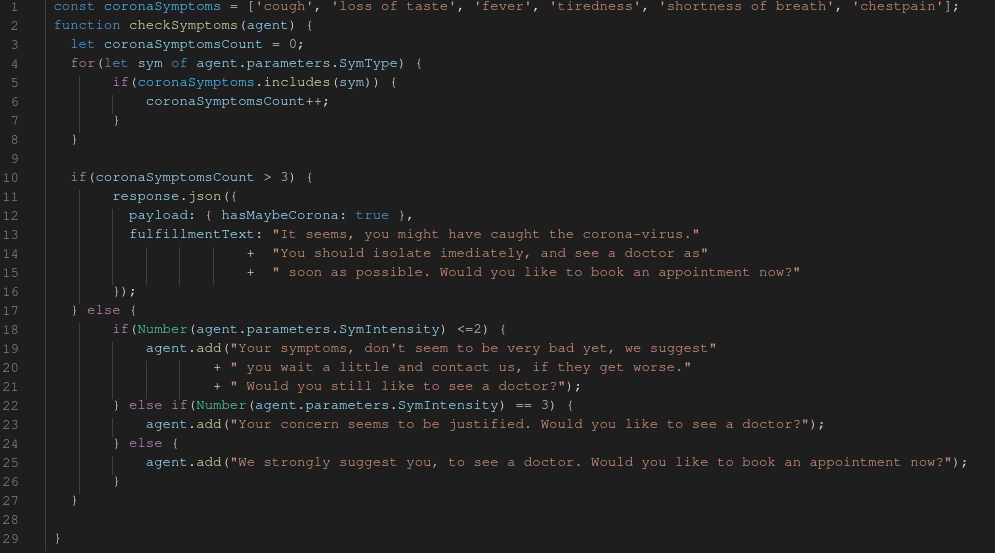
\includegraphics[width=\linewidth]{checkSymptoms.png}
            	    \caption{checkSymptoms Funktion}
	            	\label{fig:checksymptomsfunction}
	            \end{center}
    	    \end{figure}
    	    
		\paragraph{}
            Auf den Zeilen 3 bis 8 werden die angegebenen Symptome mit dem Array \emph{coronaSymptoms} verglichen und gezählt.
            Auf Zeile 10 wird überprüft, ob die Anzahl der auf Corona-Symptome passenden Symptome grösser als 3 ist. Falls dies
            der Fall ist - wird unabhängig der anderen Parametern - eine entsprechende Nachricht zurückgesandt, welche den Benutzer über
            diesen Umstand informiert und ihm vorschlägt, sich zu isolieren, sowie sich testen zu lassen.

		
		\newpage
		

        \paragraph{}
            Besteht kein Verdacht auf das Corona-Virus, so ist die Symptomstärke (\emph{"symtom\_intensity"}) ausschlaggebend für die Antwort:
            \begin{itemize}
                \item \textbf{Intensität <= 2:} Die Symptome scheinen nicht schlimm zu sein. Dem Benutzer wird geraten abzuwarten und bei
	                Verschlimmerung des Zustands einen Arzt aufzusuchen. Der Benutzer wird gefragt, ob er dennoch einen Arzttermin buchen
                    möchte
                \item \textbf{Intensität = 3:} Der Benutzer wird gefragt, ob er einen Arzttermin buchen möchte.
                \item \textbf{Intensität > 3:} Dem Benutzer wird angeraten einen Arzt aufzusuchen. Er wird gefragt, 
                	ob er einen entsprechenden Termin buchen möchte.
            \end{itemize}

        \paragraph{}
            Alle Antworten resultieren in der Frage, ob der Benutzer einen Arzttermin buchen möchte. Mit den Intents 
            \emph{check\_symptoms - yes} und \emph{check\_symptoms - no} (siehe: Abbildung \ref{fig:intentslist}) wird die Antwort des
            Benutzers abgefangen. Während \emph{check\_symptoms - no} zu einer Verabschiedungsantwort führt, fragt 
            \emph{check\_symptoms - yes} direkt, wann der Termin stattfinden soll.

    \subsection{Termin buchen}
        \paragraph{}
            Der Intent \emph{check\_symptoms - yes - time} fängt die Antwort des vorgehenden Intents (Frage nach Terminzeit) direkt ab 
            und löst im Webhook eine weitere Methode aus (siehe: Abbildung \ref{fig:handleappointmentfunction}).
	        \begin{figure}[h!]
    	        \begin{center}
        	        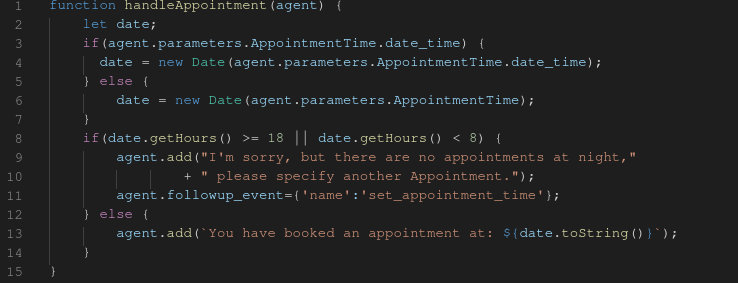
\includegraphics[width=0.7\linewidth]{handleAppointmentFunction.png}
					\caption{handleAppointment Funktion}
	            	\label{fig:handleappointmentfunction}
	            \end{center}
    	    \end{figure}

        \paragraph{}
            Die ersten 7 Zeilen der Funktion kümmern sich um das Parsen des Datums. Da dieses nicht immer gleich daher kommt,
            musste ein wenig Logik zur Überprüfung der Daten implementiert werden. Zeile 8 prüft, ob die Uhrzeit zwischen 08:00
            und 20:00 Uhr liegt. Alles zwischen diesen zwei Zeitpunkten ist als gültige Uhrzeit definiert und führt dazu, dass die
            Buchung auf Zeile 13 bestätigt wird. Der Dialog ist hiermit beendet. Liegt die Zeit allerdings ausserhalb des gültigen
            Bereichs, wird auf den Zeilen 9 und 10 eine Fehlernachricht zurückgegeben und nach einer neuen Zeit gefragt.
            Auf Zeile 11 wird als Folge-Intent das Event \emph{set\_appointment\_time} definiert. Dieses Event zeigt auf denselben 
            Intent, auf dem wir gerade operieren (\emph{check\_symptoms - yes - time}). Die Terminbuchung wird also wiederholt, bis
            eine gültige Zeit für den Termin angegeben wird. 
	        \begin{figure}[h!]
    	        \begin{center}
        	        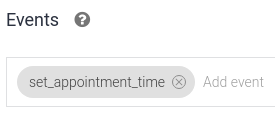
\includegraphics[width=0.35\linewidth]{eventSetting.png}
					\caption{Eventeinstellung für die Schleifenlogik}
            		\label{fig:eventSetting}
	            \end{center}
    	    \end{figure}


\newpage


\section{Java Client}
	\paragraph{}
		Der Java Client ist in die folgenden drei Bereiche aufgeteilt, welche in den nachfolgenden Unterkapitel genauer beschrieben werden:
		\begin{enumerate}
			\item Command Line Interface
			\item Dialogflow Connector
			\item Medical Assistant
		\end{enumerate}

	\subsection{Command Line Interface}
		\paragraph{}
			Beim Start des Medical Assistants im Java Client wird der User auf folgende Möglichkeiten hingewiesen:
			\begin{itemize}
				\item Input mit dem medizinischen Problem angeben
				\item "q" um den Assistenten wieder zu beenden
				\item "v" um den persönlichen medizinischen Bericht anzuschauen
			\end{itemize}
			Die logische Abfolge des Benutzerinputs, bzw. die Interaktion mit dem Dialogflow Chatbot ist analog zum beschriebenen 
			Ablauf in Abildung \ref{fig:backEndFlowChart}. Nach jeder Antwort des Chatbots können die Optionen \emph{"q"} (beenden) und 
			\emph{"v"} (Report anschauen) aufgerufen werden.
	
	\subsection{Dialogflow Connector}
		\paragraph{}
			Beim Projekttyp handelt es sich um ein Maven-Projekt. Für die Interaktion mit Dialogflow wurde das Artefakt 
			\emph{"google-cloud-dialogflow"} verwendet.
		
		\paragraph{}
			Die Einbindung, sowie die Basisimplementierung (Dialogflow Kommunikation) war bereits Bestandteil einer Übungsstunde.
			Deshalb wird dies als Vorwissen angeschaut und in diesem Report nicht weiter thematisiert. Projektspezifische Anwendungsfälle
			werden in den entsprechenden nachfolgenden Kapiteln beschrieben.
	
	\subsection{Medical Assistant Implementation}
		\subsubsection{Report}
			\paragraph{}
				Neben der Interaktion mit dem Dialogflow Chatbot ist das Hauptziel des Java Clients, dem Benutzer einen medizinischen 
				Bericht zur Verfügung zu stellen. Wenn dieser mit dem CLI Kommando \emph{"v"} abgerufen wird, ist dieser zu Beginn leer:
				\begin{figure}[h!]
					\begin{center}
        	    		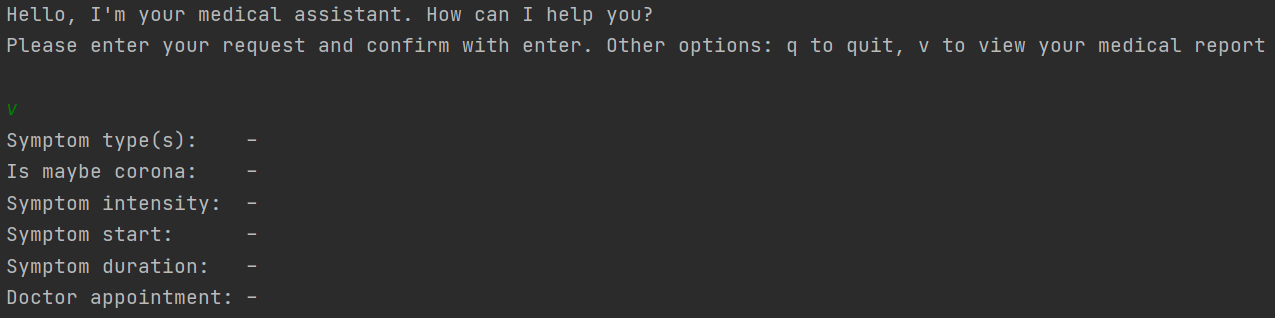
\includegraphics[width=1.0\linewidth]{JavaClient-EmptyReport.png}
		    	        \caption{Leerer medizinischer Report}
		        	    \label{fig:javaClient_emptyReport}
					\end{center}
		        \end{figure}
		        
		        
		        \newpage
		        
		        
	        	Fortlaufend - basierend auf den User-Inputs, sowie den Chatbot Antworten - wird der Report ergänzt (siehe:
	        	\ref{sssec:intent_handling}). Am Ende kann der ausgefüllte Bericht zum Beispiel folgendermassen aussehen:
				\begin{figure}[h!]
					\begin{center}
        	    		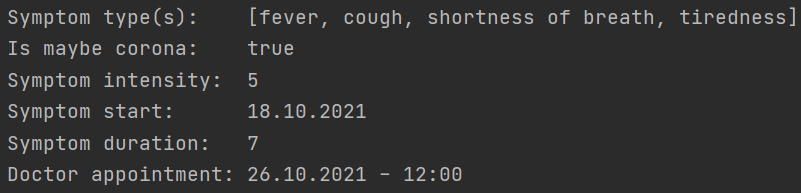
\includegraphics[width=0.8\linewidth]{JavaClient-CompletedReport.png}
		    	        \caption{Komplett ausgefüllter Beispiel-Report}
		        	    \label{fig:javaClient_completedReport}
					\end{center}
		        \end{figure}
		
		\subsubsection{Intent Handling} \label{sssec:intent_handling}
			\paragraph{}
				Die für den Java Client relevanten Intents sind \emph{"check\_symptoms"}, sowie der Folge-Intent 
				\emph{"check\_symptoms - yes - time"}. Via Switch-Case Statement werden Intent-spezifische Aktionen durgeführt,
				welche schlussendlich den medizinischen Bericht aktualisieren. \\\\
		
				\underline{\emph{Intent "check\_symptoms"}} \\
				\begin{enumerate}
					\item Via Dialogflow Backend wird dynamisch anhand der Symptome ermittelt, ob der Benutzer eventuell Corona hat.
						Diese Information wird über den Payload an den Java Client übermittelt. Das Query-Result im Java Code enthält 
						die Methode \emph{"getWebhookPayload()"}, welche den Zugriff auf den Payload als Struct ermöglicht. Auf dieser
						Datenbasis wird der Report entsprechend um das Attribut \emph{"hasMaybeCorona"} ergänzt.
						\begin{figure}[h!]
							\begin{center}
			            		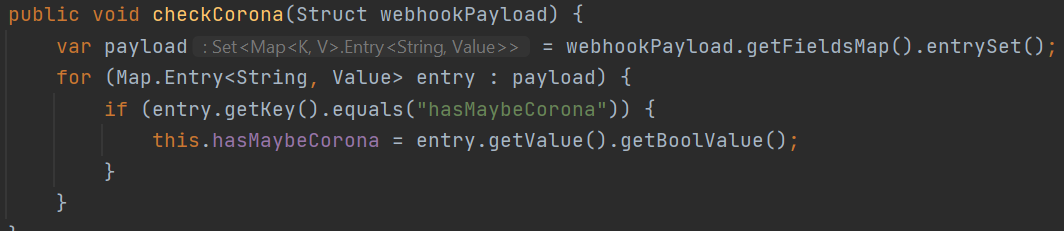
\includegraphics[width=1.0\linewidth]{JavaClient-CoronaCheck.png}
								\caption{Corona Payload zum Report hinzufügen}
								\label{fig:javaClient_coronaCheck}
							\end{center}
						\end{figure}
					
					
					\newpage
					
					
					\item Im nächsten Schritt werden alle aktualisierten Parameter auf dem Report im Java Client hinterlegt. 
						Nachfolgend ist ein Ausschnitt der Aktualisierung des ersten Parameters zu sehen. Alle anderen Parameter 
						werden im Swicht-Case Statement analog zu diesem Beispiel aktualisiert.
						\begin{figure}[h!]
							\begin{center}
			            		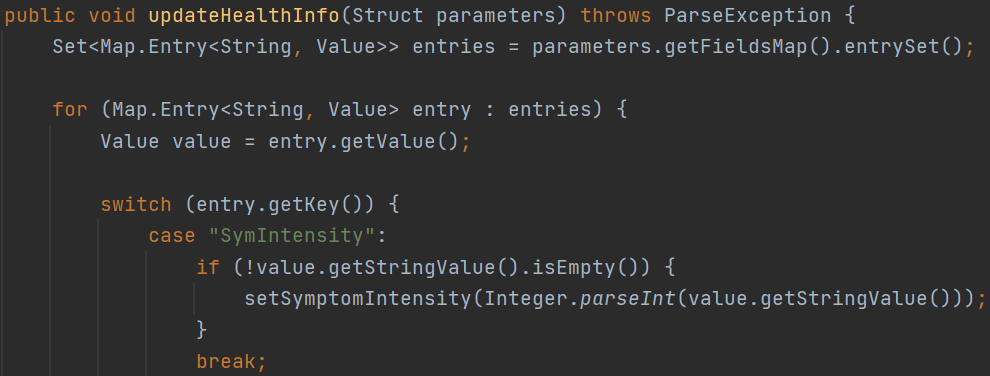
\includegraphics[width=0.9\linewidth]{JavaClient-ParameterHandling.png}
								\caption{Ausschnitt der Report Aktualisierung}
								\label{fig:javaClient_parameterHandling}
							\end{center}
						\end{figure}
				\end{enumerate}
		
		\underline{\emph{Intent "check\_symptoms - yes - time"}} \\
		\begin{enumerate}
			\item In diesem Intent wird noch der Arzttermin auf dem Report aktualisiert.
			\begin{figure}[h!]
				\begin{center}
            		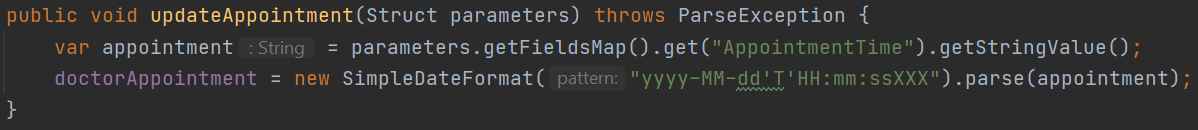
\includegraphics[width=1.0\linewidth]{JavaClient-UpdateAppointment.png}
					\caption{Arzttermin auf dem Report hinzufügen}
					\label{fig:javaClient_updateAppointment}
				\end{center}
			\end{figure}
		\end{enumerate}
	        
\newpage

\section{Diskussion}
    \subsection{Was wir gelernt haben}
        \paragraph{}
            Bei der Umsetzung dieses Projekts haben wir gelernt, dass die Dialogflow Plattform sich äusserst gut eignet, um Schnittstellen
            zwischen Menschen und Informatiksystemen zu konstruieren. Die so erschaffenen Benutzeroberflächen sind - wenn richtig umgesetzt -
            sehr intuitiv zu bedienen. Sehr viel Potential bietet diese Technologie aus unserer Sicht auch, um Menschen mit körperlichen
            Einschränkungen den Zugang zu diversen Programmen zu verschaffen. Das bekannteste Beispiel sind dabei moderne Sprachassistenten.
            
    \subsection{Limitationen}
        \paragraph{}
            Wenn man an AI denkt, geht man schnell davon aus, dass sich eine Interaktion mit einem System kaum noch von einer Interaktion 
            mit einem Menschen unterscheidet. Dies mag vielleicht in Zukunft der Fall sein, ist es aber heute noch nicht.
            
        \paragraph{}
            Dialogflow, kommt schnell an seine Grenzen, wenn man den Chat-Bot mit ungenauen oder zusätzlichen (unnötigen) Informationen
            beliefert, für die er nicht trainiert wurde.
            
    \subsection{Erweiterungsmöglichkeiten unserer Arbeit}
        \paragraph{}
            Um die Aufnahme der Informationen weiter zu verbessern, könnte der Satz an Trainingssätzen erweitert werden, sodass es weniger
            häufig zu Missverständnissen durch einfache Schreibfehler kommt.
            
        \paragraph{}
            Weiter könnte man unseren Chatbot durch folgende Features erweitern, um ihn für einen produktiven Einsatz vorzubereiten:
            \begin{itemize}
                \item Buchungssystem mit persistenten Daten und Konfliktauflösung, um doppelte Terminbuchungen zu verhindern.
                \item Automatische Zuweisung von Patienten an Ärzte mit unterschiedlichen Spezialisierungen, basierend auf den angeggebenen
                	Symptomen.
                \item Implementation eines Webinterfaces oder Interface mit einem Sprachassistenten.
                \item Integration in Chat-App, um eine vereinfachte Kommunikation zu ermöglichen (z. B. Facebook Messenger oder Telegram)
            \end{itemize}

\end{document} 
